\documentclass[12pt]{article}
\usepackage[utf8]{inputenc}
\usepackage{amsmath}
\usepackage{amssymb}
\usepackage{graphicx}
\usepackage{hyperref}
\usepackage{geometry}
\geometry{a4paper, margin=1in}
\usepackage{xcolor}
\usepackage{booktabs}

\title{\textbf{Deconstructing Diffusion Models \\ Part 3: Watching Noise Become Art}}
\author{Sovesh Mohapatra}
\date{\today}

\begin{document}
\maketitle

\section*{Introduction}
In Part 1, we outlined the math of the forward corruption process. In Part 2, we built the UNet, the time embeddings, and the training loop in pure PyTorch.

Now, we reap the rewards: generating novel data from pure static. We trained our custom DDPM on the MNIST dataset for 15 epochs. While classifying MNIST is trivial for modern deep learning, \textit{generating} MNIST from scratch using a continuous Markov chain is a visually stunning demonstration of how state-of-the-art architectures (like DALL-E and Sora) learn the fundamental distribution of data.

\section*{The Training Process}

Our primary objective is predicting the Gaussian noise vector $\epsilon$ that was added to an image at some random timestep $t$. The loss is the Mean Squared Error between the actual noise and the network's prediction.

\begin{figure}[h]
    \centering
    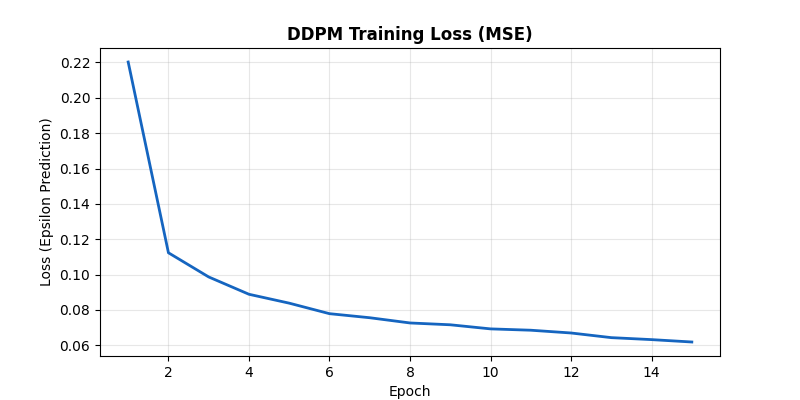
\includegraphics[width=0.8\textwidth]{training_loss.png}
    \caption{The MSE loss of the UNet predicting the added Gaussian noise over 15 epochs. The smooth downward trend confirms the network is successfully learning the noise structure across all $T=1000$ timesteps.}
    \label{fig:loss}
\end{figure}

The UNet learns very quickly to separate structure from static. Note that because $t$ is sampled uniformly $[0, T]$, the network is forced to learn how to denoise an image at every possible stage of corruption—from a mostly clear digit with light grain ($t \approx 10$) to pure TV fuzz ($t \approx 1000$).

\section*{Generation: The Denoising Trajectory}

To generate a new image, we start with a tensor of pure Gaussian noise, $\mathcal{N}(0, \mathbf{I})$. We feed this into the network with $t=1000$. The network guesses the noise, we subtract a fraction of it, inject a small amount of new regularizing noise, and step to $t=999$. We recurse this process 1,000 times.

Figure~\ref{fig:trajectory} shows this beautiful, slow resolution of order from chaos:

\begin{figure}[h]
    \centering
    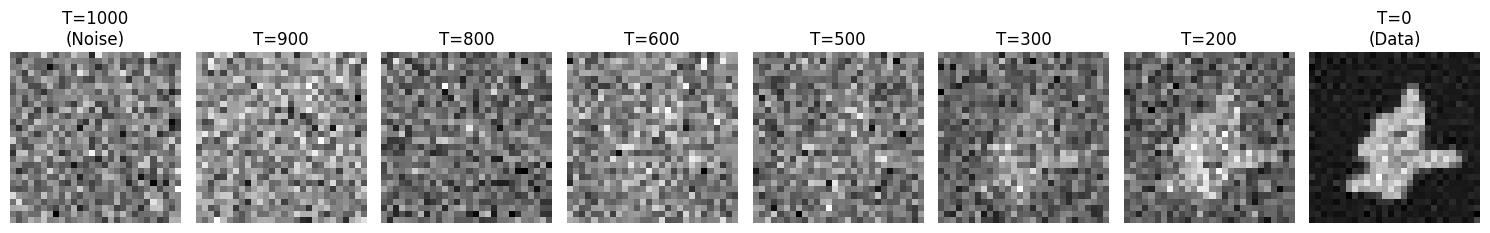
\includegraphics[width=0.95\textwidth]{denoising_trajectory.png}
    \caption{The reverse process in action. Starting from pure isotropic Gaussian noise at $T=1000$, the network iteratively strips away predicted noise. Notice how the shape remains highly ambiguous until around $T=400$, after which the high-frequency details of the specific digit crystallize.}
    \label{fig:trajectory}
\end{figure}

\section*{The Final Generation Grid}

After running the full 1,000-step reverse process for a batch of 32 independent noise seeds, the network produces a diverse array of handwritten digits (Figure~\ref{fig:grid}).

\begin{figure}[h]
    \centering
    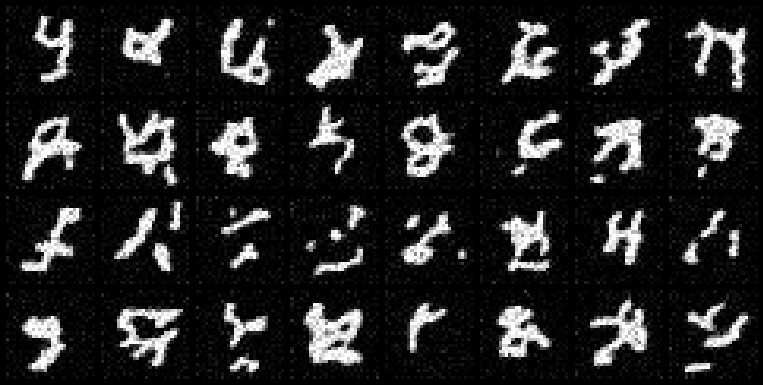
\includegraphics[width=0.8\textwidth]{generate_grid.png}
    \caption{A 4x8 grid of generated MNIST digits. Unlike an Autoencoder, a Diffusion Model learns a fully expressive mapping from the isotropic Gaussian generic prior to the complex multi-modal data distribution. None of these exact digits exist in the training set.}
    \label{fig:grid}
\end{figure}

The generated digits display remarkable variety in slant, thickness, and stylistic form—proving the network didn't just memorize the training set, but actually learned the continuous latent manifold of the digits.

\section*{Conclusion}

Diffusion models have revolutionized generative AI because they solve a critical problem that GANs and VAEs struggled with: stable, high-fidelity mapping from a simple prior (Gaussian noise) to a complex data distribution.

By breaking the generation process down into 1,000 tiny, easily learned denoising steps, DDPMs replace the brittle adversarial training of GANs with a stable, mathematically rigorous maximum likelihood (ELBO) objective.

We built this entirely from scratch in PyTorch—no external diffusion libraries, no pre-trained weights. By seeing the raw UNet predict $\epsilon$ and watching the $T \to 0$ loop resolve into a digit, we demystify the core algorithm powering today's most advanced AI systems.

\vspace{1em}
\noindent \textit{Thank you for following this 3-part ``Build in Public'' series on Diffusion Models. Stay connected on LinkedIn for future architectural tear-downs!}

\end{document}
